\documentclass[12pt, 
hyperref={colorlinks=true, linkcolor=blue, urlcolor=cyan},dvipsnames]{beamer}
\usetheme{default} 

\setbeamertemplate{navigation symbols}{} %gets rid of navigation symbols
\setbeamertemplate{footline}{} %gets rid of bottom navigation bars
\setbeamertemplate{footline}[page number]{} %use this for page numbers

\setbeamertemplate{itemize items}[circle] %round bullet points
\setlength\parskip{10pt} % white space between paragraphs

\usepackage{wrapfig}
\usepackage{subfig}
\usepackage{setspace}
\usepackage{enumerate}
\usepackage{graphicx}
\usepackage{amsmath}
\usepackage{amsfonts}
\usepackage{amssymb}
\usepackage{amsthm}
\usepackage[UKenglish]{isodate}
\usepackage{verbatim}
\usepackage{xcolor}
\cleanlookdateon

% new amber color
\definecolor{amber}{rgb}{1.0, 0.75, 0.0}

\DeclareMathOperator{\argmin}{argmin}

% the preamble
\title{BIOST 311: \\ Regression Methods for the Health Sciences}
\author{Kelsey Grinde and Brian Williamson}
\institute{UW Biostatistics}
\date{Spring 2018}

\begin{document}
% title slide
\begin{frame}
\titlepage\thispagestyle{empty}
\end{frame}

% make it 1.something
\setbeamertemplate{footline}{%
  \raisebox{5pt}{\makebox[\paperwidth]{\makebox[120pt]{\scriptsize Last updated \today}\hfill\makebox[20pt]{\scriptsize 3.\insertframenumber~~}}}}  \newcounter{chap3}{\value{1}}
\setcounter{framenumber}{\value{chap3}}

\begin{frame}
\frametitle{CHAPTER 3: SURVIVAL ANALYSIS}
By the end of Chapter 3, you should be able to: \vspace{-0.3cm}

\begin{itemize}
\item Determine if a variable has been \textcolor{BurntOrange}{right-censored}
\item Discuss the \textcolor{red}{drawbacks} of treating a right-censored variable as binary or continuous
\item \textbf{Interpret Kaplan-Meier curves}, and create them in \texttt{R}
\item \textbf{Implement and interpret} a logrank test for equating survival curves
\item \textbf{Formulate a regression model} given a scientific or statistical question about a right-censored outcome
\item \textbf{Interpret the coefficients} for a (simple or multiple) proportional hazards regression model
\item \textbf{Interpret confidence intervals and p-values} for proportional hazards regression coefficients
\item Use \texttt{R} to fit a proportional hazards regression model and create figures/tables to support your regression analysis
\end{itemize}

\end{frame}

\section{Censored outcomes}
\begin{frame}
\frametitle{SECTION 1: CENSORED OUTCOMES}
Up to this point, we have focused on questions involving \textcolor{blue}{quantitative} or \textcolor{BurntOrange}{binary} outcomes: 
\begin{itemize}
\item Is lung function (\textcolor{blue}{FEV}) associated with smoking, after adjusting for age, height, and sex?
\item Is cognitive function (\textcolor{blue}{DSST score}) associated with alcohol use, adjusting for age, sex, and education?
\item Is \textcolor{BurntOrange}{diabetes} associated with BMI, after adjusting for sex?
\end{itemize}
\end{frame}

\begin{frame}
\frametitle{SECTION 1: CENSORED OUTCOMES}
However, we are often interested in scientific questions that involve \textcolor{blue}{time-to-event} outcomes:
\begin{itemize}
\item Is \textcolor{blue}{time to first seizure post operation to remove a brain tumor} associated with pre-operation case review by an epileptologist, in children with both epilepsy and brain tumor?
\item Is \textcolor{blue}{time to promotion for university faculty members} associated with sex?
\item Is \textcolor{blue}{time to death from any cause} associated with serum levels of C reactive protein?
\end{itemize}
\end{frame}

\begin{frame}
\frametitle{Characteristics of survival data}
{\fontsize{10pt}{7.2}\selectfont
Sample of the observed times until first severe panic attack (in weeks):
\hspace*{-1cm}\begin{tabular}{|c|c|c|c|c|c|c|c|c|c|}
\hline
\textcolor{blue}{meditation group} & 14.29 & 7.74 & 21 & 25.18 & 2.83 & 17.57 & 19.13 & 0.14  \\
\hline
control group & 21 & 3.94 & 7.77 & 6.54 & 24 & 12.55 & 21.29 & 3.58 \\
\hline
\end{tabular}
}

We wish to study whether \textcolor{blue}{meditation} prolongs the \textbf{time until a severe panic attack} in patients suffering from a panic disorder.

To address this question, we: \vspace{-0.3cm}
\begin{itemize}
\item recruit 200 patients and randomize them to meditation or placebo;
\item follow each patient until their first severe panic attach post recruitment;
\item and compare the mean time until a severe panic attack in each group with a t-test
\end{itemize}

\end{frame}

\begin{frame}
\frametitle{Characteristics of survival data}
\centering
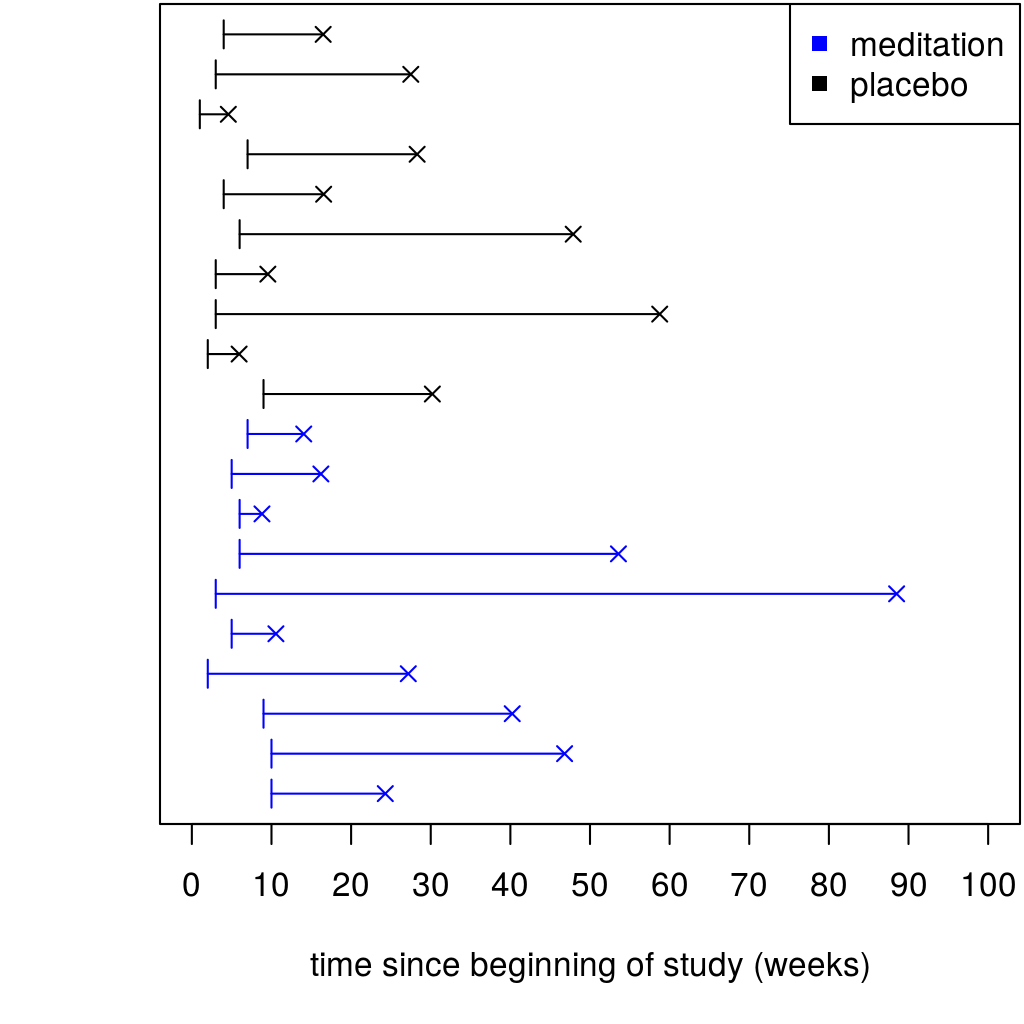
\includegraphics[width=0.8\textwidth]{figs/meditation_observed_study_time.png}
\end{frame}

\begin{frame}
\frametitle{Characteristics of survival data}
\centering
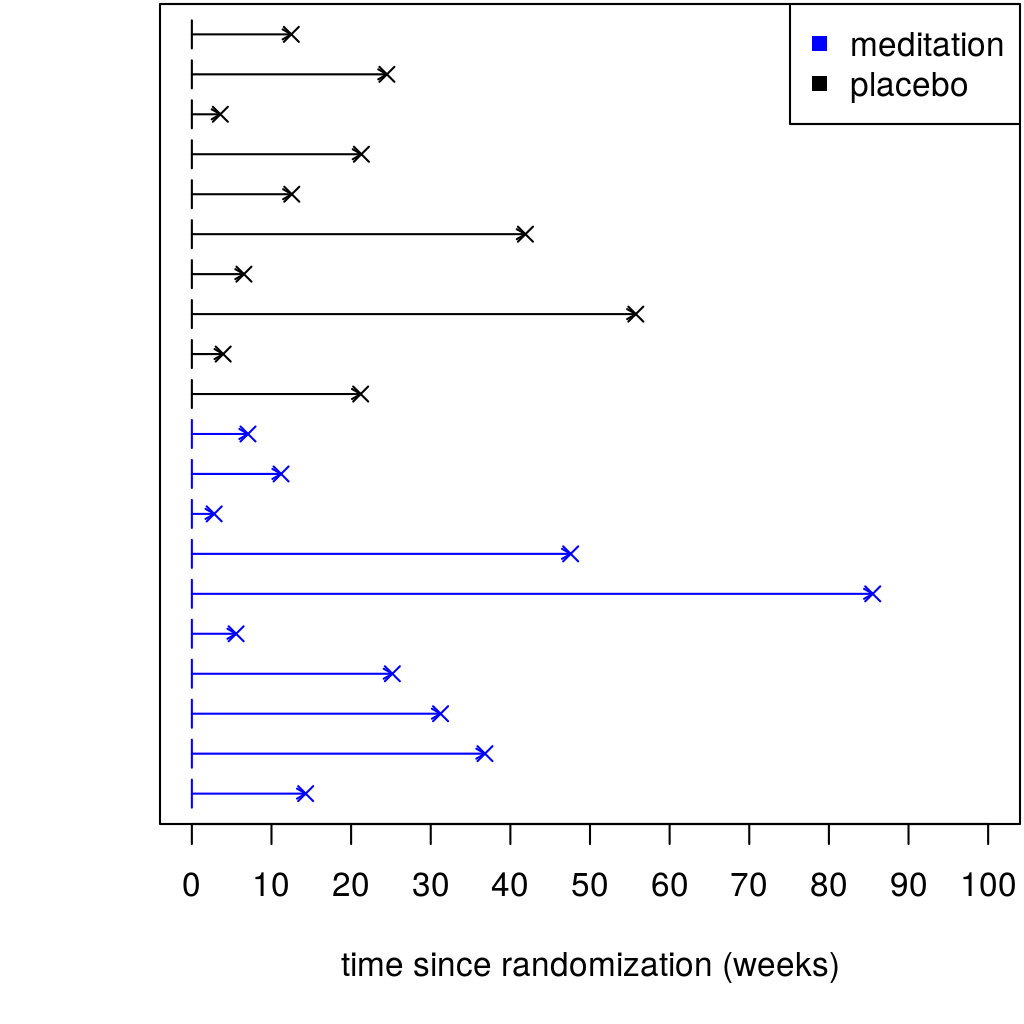
\includegraphics[width=0.8\textwidth]{figs/meditation_observed_rand_time.png}
\end{frame}

\begin{frame}
\frametitle{Characteristics of survival data}
In this hypothetical study, we were able to record the actual occurrence time \textcolor{blue}{for each participant}.

Is this typical of human studies? \pause \textcolor{red}{No!}

Why? \pause Some common reasons are:
\begin{itemize}
\item the study ended (e.g., after 30 weeks) and some participants had not yet had a severe panic attack (\textbf{administrative censoring})
\item the participant left the study before having had a severe panic attack (\textbf{loss to follow-up})
\end{itemize}

These all lead to \textbf{right-censored} data, where rather than knowing the value exactly, we know that the value exceeds some cutoff.
\end{frame}

\begin{frame}
\frametitle{Characteristics of survival data}
\centering
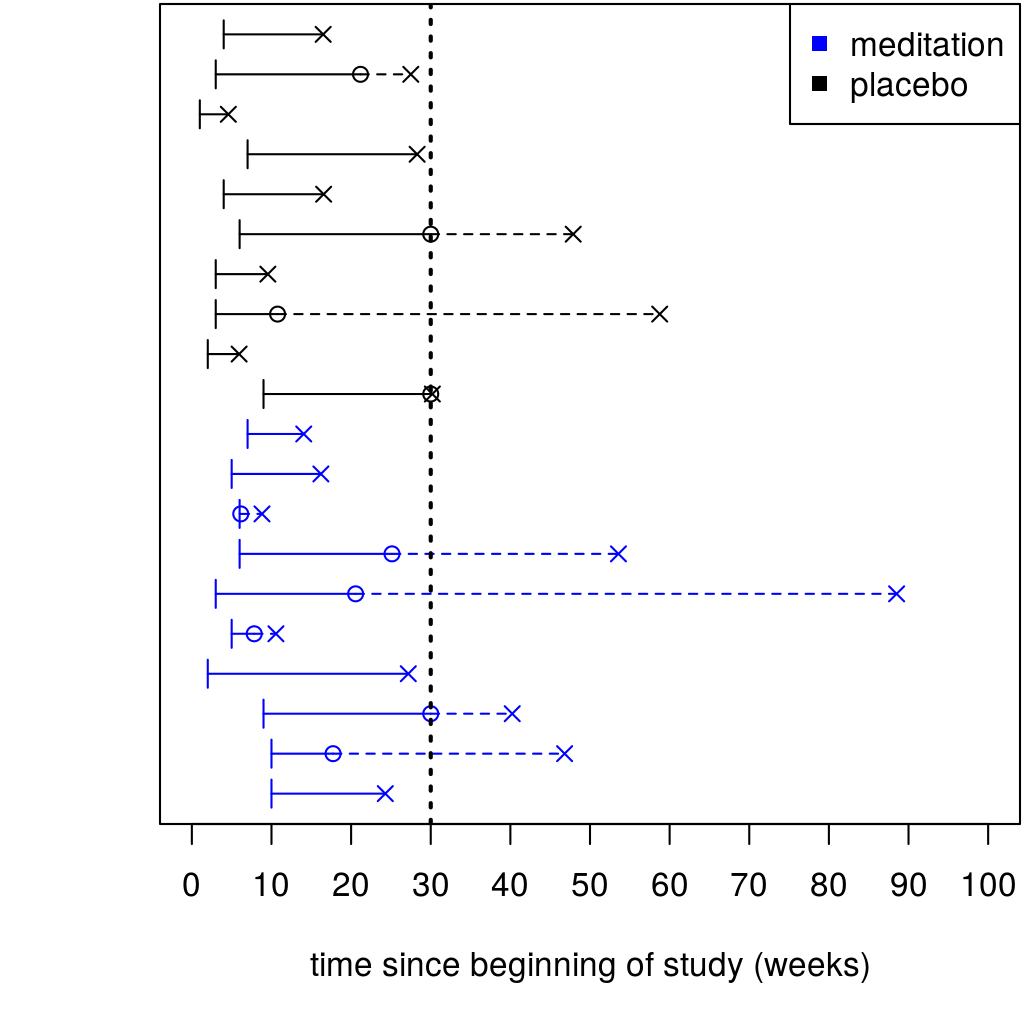
\includegraphics[width=0.8\textwidth]{figs/meditation_censored_study_time.png}
\end{frame}

\begin{frame}
\frametitle{Characteristics of survival data}
\centering
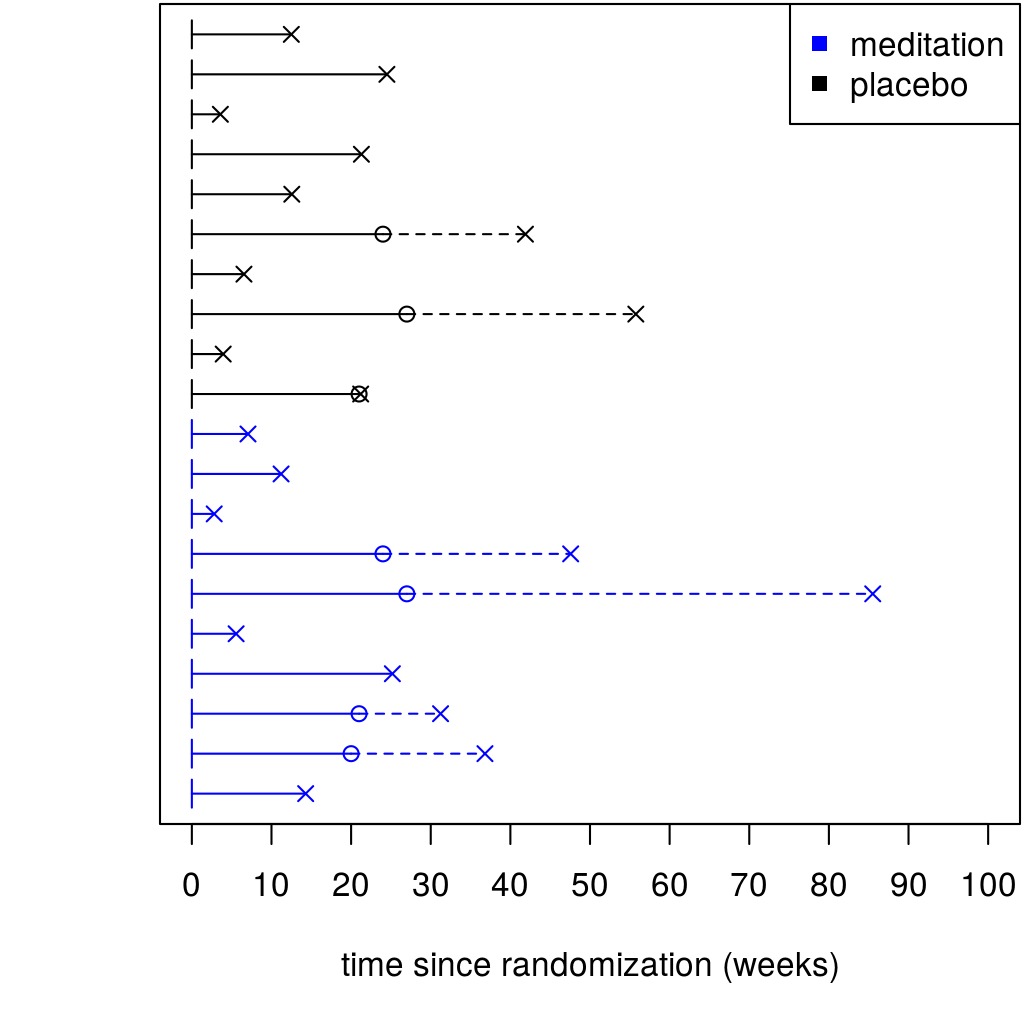
\includegraphics[width=0.8\textwidth]{figs/meditation_censored_rand_time.png}
\end{frame}

\begin{frame}
\frametitle{Characteristics of survival data}
{\fontsize{10pt}{7.2}\selectfont
The data can be represented as:
\hspace*{-1cm}\begin{tabular}{|c|c|c|c|c|c|c|c|c|c|}
\hline
\textcolor{blue}{meditation group} & 14.29  & \textcolor{red}{7.74+} & \textcolor{red}{21.00+} & 25.18  &  \textcolor{red}{2.83+} & \textcolor{red}{17.57+} & \textcolor{red}{19.13+} &  \textcolor{red}{0.14+}  \\
\hline
control group & \textcolor{red}{21.00+} &  \textcolor{red}{3.94+} &  \textcolor{red}{7.77+} &  6.54  & \textcolor{red}{24.00+} & 12.55  & 21.29 &  3.58 \\
\hline
\end{tabular}
}

\vspace{-0.6cm}
{\small
Should we treat these incompletely observed times as missing data? Should we throw them out? \pause \textcolor{red}{Either of these is a bad idea!} \vspace{-0.3cm}

\begin{itemize}
\item These observations contain valuable information:
{\scriptsize
\begin{itemize}
\item \textcolor{red}{20+}: the participant did not experience a severe panic attack before 20 weeks
\item their actual time until the first severe panic attack must be in the interval $(20, +\infty)$
\end{itemize}
}
\item These participants are not representative of the whole study population: valid estimation and inference when excluding missing data (which we have done so far) assumes that the people excluded are ``similar to'' the people still in the data (\textbf{missing completely at random})
\end{itemize}
}
\end{frame}

\begin{frame}
\frametitle{Characteristics of survival data}
Close or put away your notes and laptops. Then answer the following questions, paying attention your thought process (you will hand in your responses):
\begin{enumerate}
\item Are those with smaller or larger times more likely to be censored? Why?
\item Systematically excluding censored times could lead to \textcolor{red}{biased estimates}. Would this lead to an overestimation or an underestimation of the mean time until severe panic attack? Why?
\end{enumerate}

\end{frame}

\begin{frame}
\frametitle{Characteristics of survival data}
\begin{enumerate}
\item Are those with smaller or larger times more likely to be censored? Why?
\item[] \textcolor{blue}{Those with \textbf{larger times} are more likely to be censored; we only get to observe these people for a comparatively small amount of time, so we may miss their event}
\item Systematically excluding censored times could lead to \textcolor{red}{biased estimates}. Would this lead to an overestimation or an underestimation of the mean time until severe panic attack? Why?
\item[] \textcolor{blue}{\textbf{Underestimation}: if we exclude censored times, then we are effectively excluding these people with potentially longer times, and losing all of this information!}
\end{enumerate}

\end{frame}

\begin{frame}
\frametitle{Characteristics of survival data}
Sampling distribution of times in participants who become censored or uncensored, and the overall target population:\vspace{-0.4cm}
\begin{center}
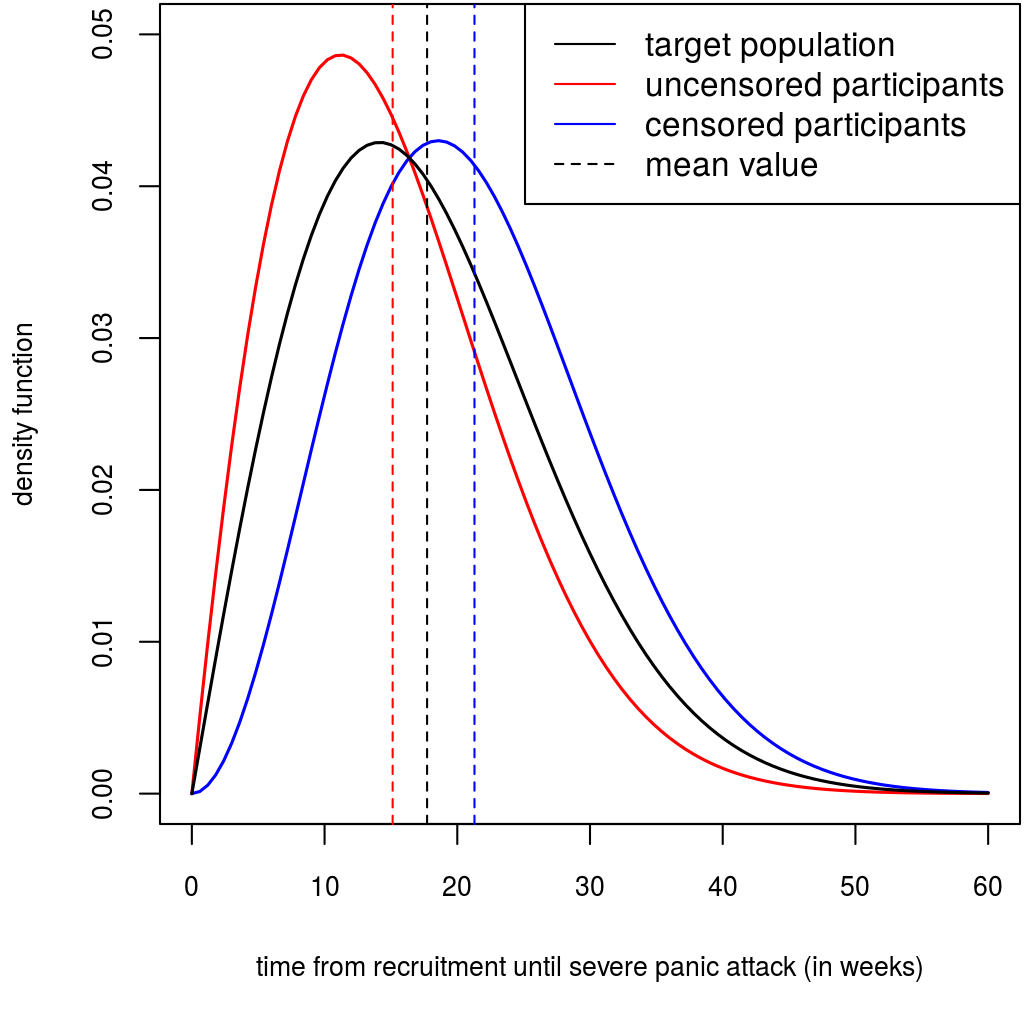
\includegraphics[height=0.8\textheight]{figs/meditation_density_versus_obs_time.png}
\end{center}
\end{frame}

\begin{frame}
\frametitle{Characteristics of survival data}
\textbf{Survival analysis} is the branch of statistics concerned with the analysis of \textbf{time-to-event data}.

Often, the goals of a survival analysis are to:
\begin{itemize}
\item describe the distribution of a time-to-event variable
\item compare the time-to-event distribution in different subpopulations
\item investigate the relationship between explanatory variables and the time-to-event distribution
\end{itemize}

Even when our time-to-event data do not truly mean survival (e.g., time to first severe panic attack), we still use the term ``survival''.
\end{frame}

\begin{frame}
\frametitle{Characteristics of survival data}
Why is time-to-event data special? Why can we not use standard methods? \vspace{-0.5cm}
\begin{itemize}
\item A time-to-event variable is positive and generally skewed
\item To appropriately define a time-to-event, we must specify:
{\scriptsize
\begin{itemize}
\item initiating event --- e.g., birth, recruitment into study, onset of disease
\item terminating event --- e.g., death, onset of disease
\item time scale --- e.g., calendar time, number of transfusions
\end{itemize}
}
\item Time-to-event data are generally observed subject to some incompleteness, of which \textbf{censoring} is a major type
\item Throwing away incomplete data generally results in
{\scriptsize
\begin{enumerate}
\item a loss of information (and increase in estimation uncertainty)
\item biased estimation procedures (most important!)
\end{enumerate}
}
\end{itemize}

\end{frame}

\begin{frame}
\frametitle{Characteristics of survival data}
A time-to-event variable is said to be \textbf{censored} if rather than being known exactly, it is known to lie in some set of values.

In this course, we will focus on \textbf{right censoring}, where we only know that the event occurred after the censoring point.

Right-censored data are the most common type of censored data found in applications!
\end{frame}

% risk set, plus movie
\begin{frame}
\frametitle{Characteristics of survival data}
Key concept: the \textbf{risk set}.

\textbf{Risk set at time $t$}: the collection of participants that \textcolor{blue}{could have experienced} their first severe panic attack at time $t$; in other words, those who were still at risk at time $t$.
\vspace{-0.3cm}
\begin{align*}
\textbf{fraction at risk at time } t = & \frac{\textbf{size of risk set at time } t}{\textbf{total sample size}}.
\end{align*}

A few observations:\vspace{-0.3cm}
\begin{itemize}
\item participants \textcolor{blue}{exit} the risk set either when they \textcolor{Aquamarine}{experience a severe panic attack} or when they \textcolor{red}{become right-censored}
\item with right-censored data, all participants are in the risk set at time 0 and the risk set necessarily shrinks over time
\item the \textcolor{blue}{size of the risk set} and the \textcolor{blue}{characteristics of its members} will be critical in survival analysis
\end{itemize}
\end{frame}

\begin{frame}
\frametitle{Characteristics of survival data}
\begin{center}
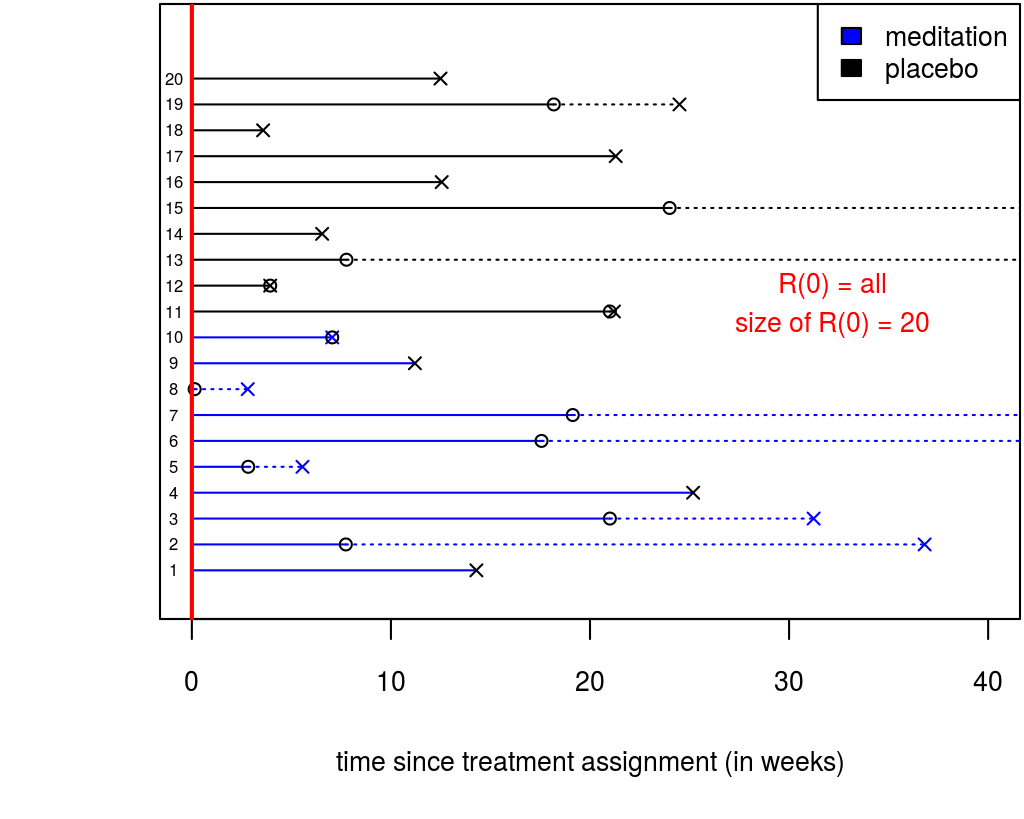
\includegraphics[height=0.8\textheight]{figs/risk_set_movie_0.png}
\end{center}
\end{frame}

\begin{frame}
\frametitle{Characteristics of survival data}
\begin{center}
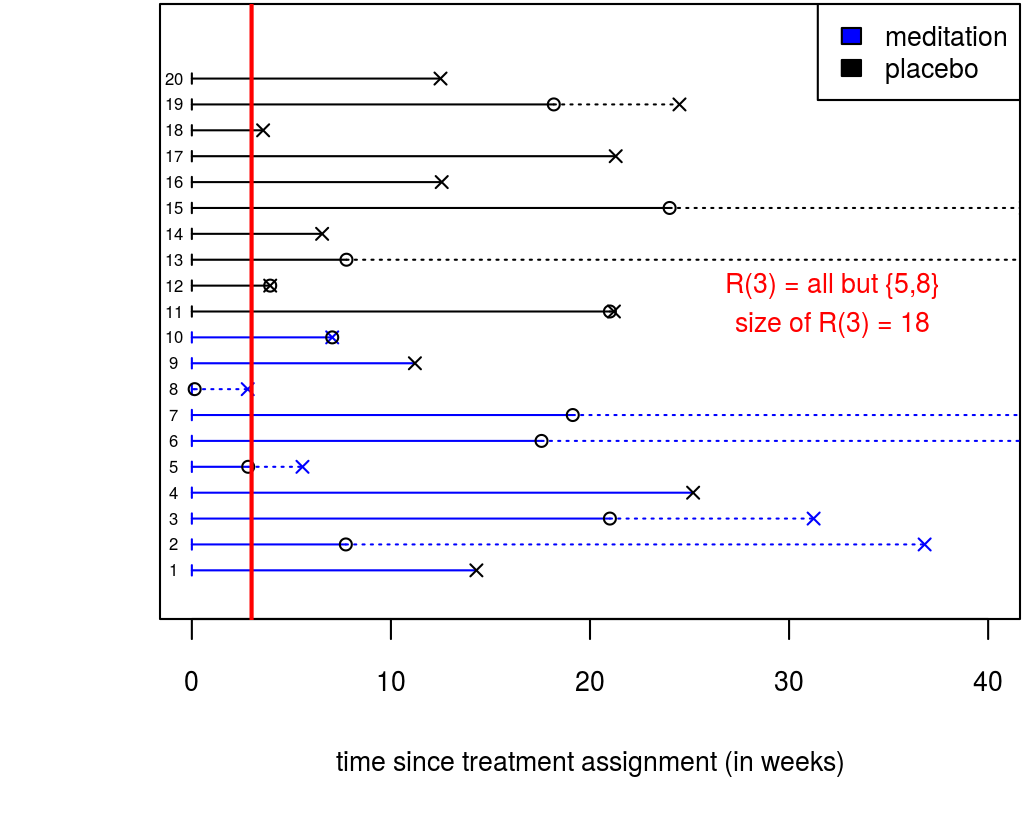
\includegraphics[height=0.8\textheight]{figs/risk_set_movie_1.png}
\end{center}
\end{frame}

\begin{frame}
\frametitle{Characteristics of survival data}
\begin{center}
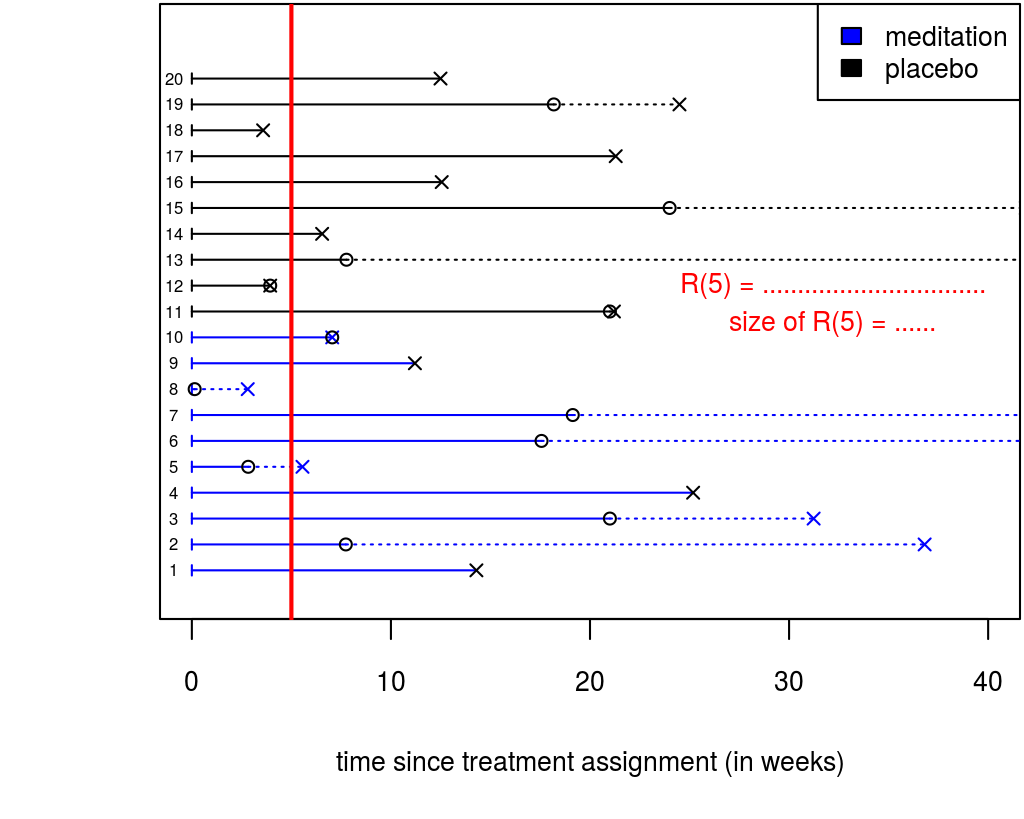
\includegraphics[height=0.8\textheight]{figs/risk_set_movie_2.png}
\end{center}
\end{frame}

\begin{frame}
\frametitle{Characteristics of survival data}
\begin{center}
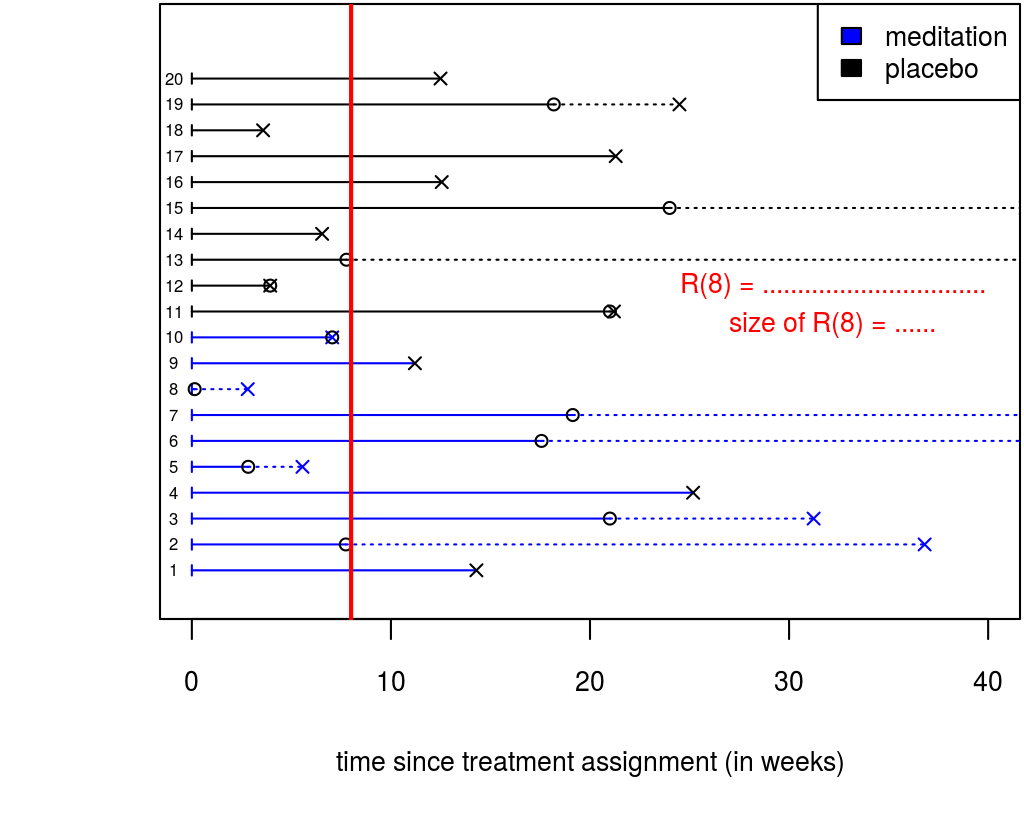
\includegraphics[height=0.8\textheight]{figs/risk_set_movie_3.png}
\end{center}
\end{frame}

\begin{frame}
\frametitle{Characteristics of survival data}
\begin{center}
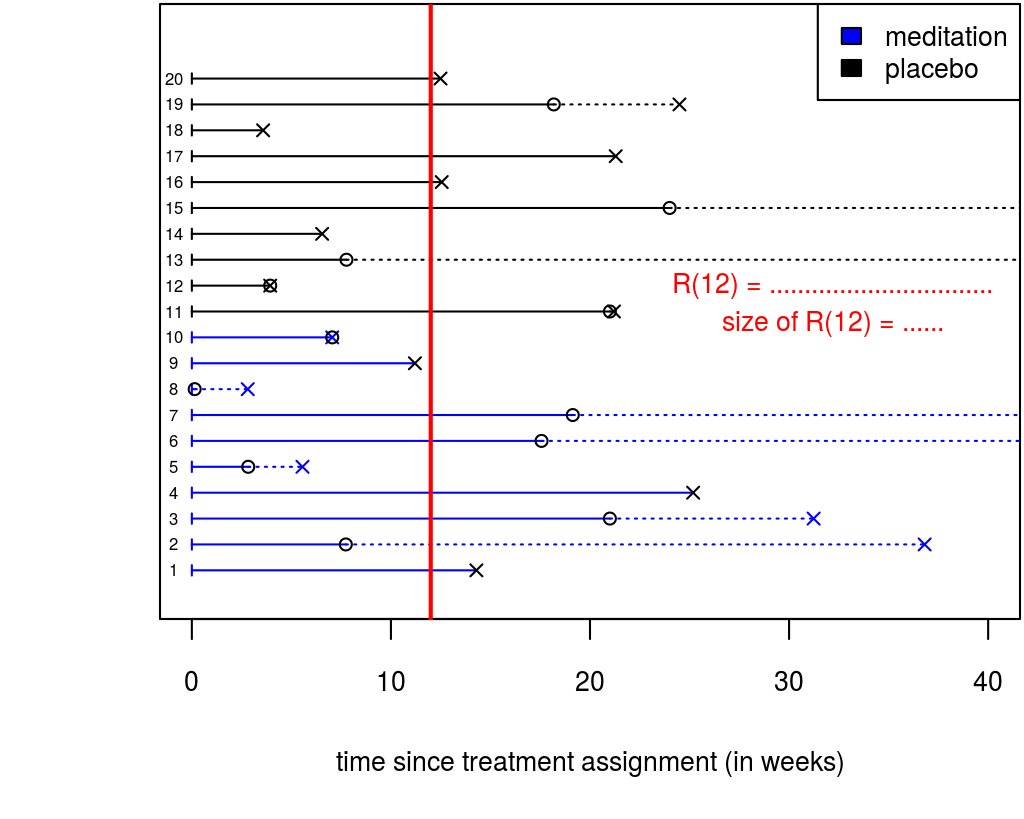
\includegraphics[height=0.8\textheight]{figs/risk_set_movie_4.png}
\end{center}
\end{frame}

\begin{frame}
\frametitle{Characteristics of survival data}
\begin{center}
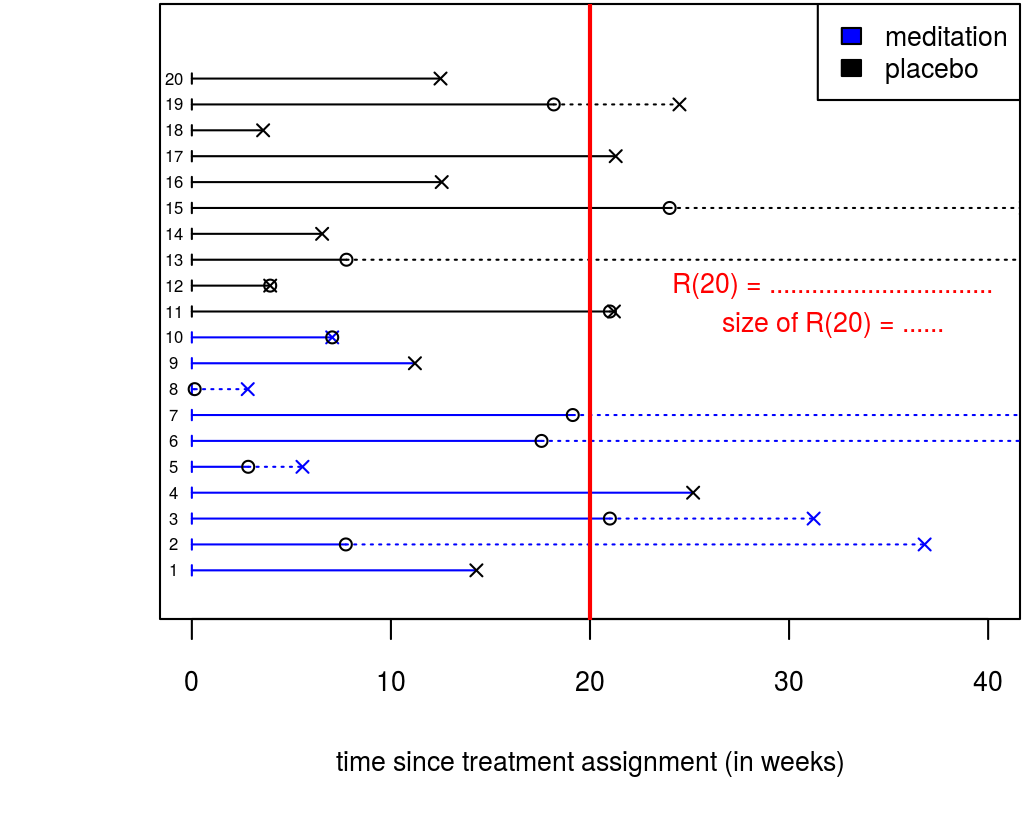
\includegraphics[height=0.8\textheight]{figs/risk_set_movie_5.png}
\end{center}
\end{frame}

\begin{frame}
\frametitle{Characteristics of survival data}
\begin{center}
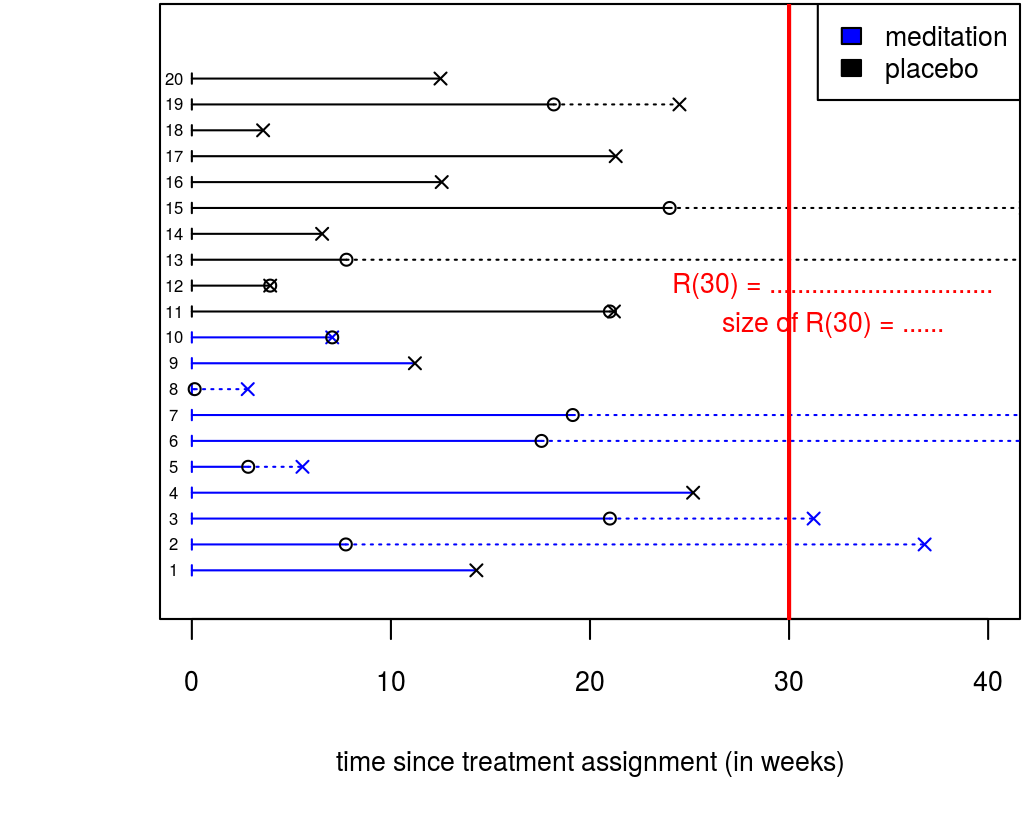
\includegraphics[height=0.8\textheight]{figs/risk_set_movie_6.png}
\end{center}
\end{frame}

\begin{frame}
\frametitle{Characteristics of survival data}
\begin{center}
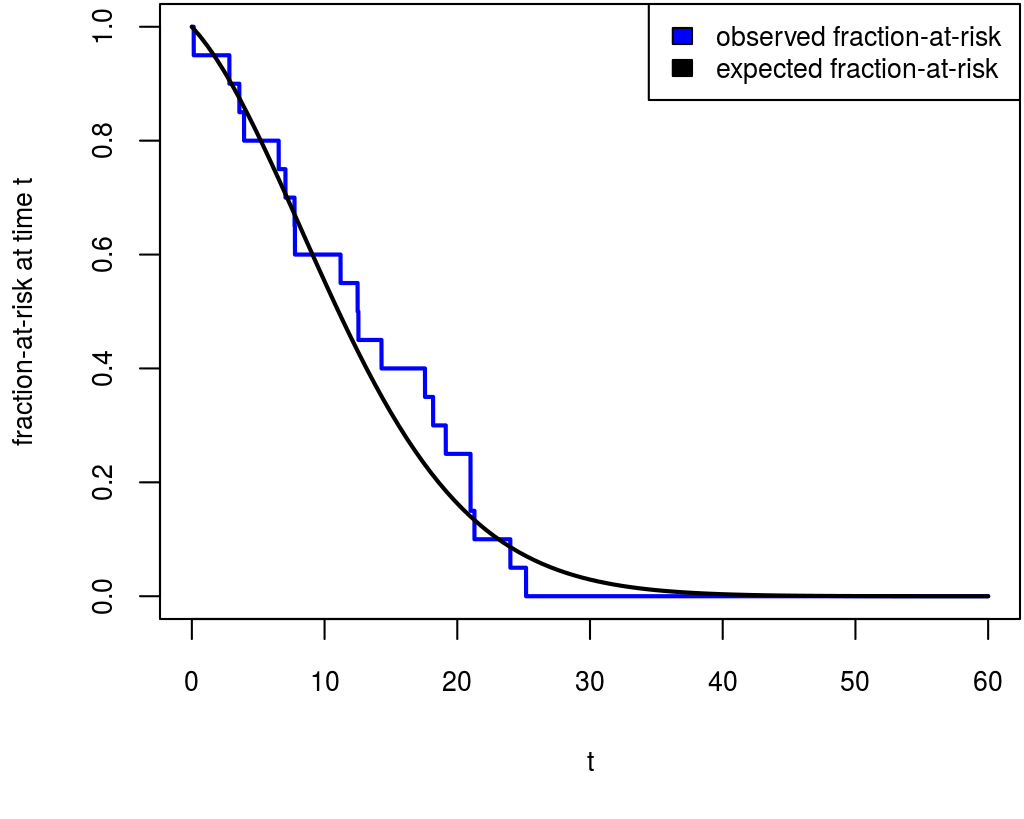
\includegraphics[height=0.8\textheight]{figs/risk_set.png}
\end{center}
\end{frame}
% uninformative censoring, with examples (from Anna)

\begin{frame}
\frametitle{Characteristics of survival data}
The assumption of \textbf{independent (or uninformative) censoring} is \textcolor{red}{critical} to the vast majority of methods available in survival analysis.

A participant's \textbf{time-to-event} and potential \textbf{censoring time} should be \textbf{independent} of one another.

What does that mean? \pause \textit{Individuals in the risk set at time $t$ must be \textbf{similar} to members of the target population who haven't experienced their first severe panic attack by time $t$.}

When is this reasonable? \vspace{-0.3cm}
\begin{itemize}
\item Participants are censored because the study ended? \pause \textcolor{blue}{Yes!}
\item Participants exited the study because their panic disorder became disabling? \pause \textcolor{red}{No!}
\item Participants exited the study because their panic disorder dissipated? \pause \textcolor{red}{No!}
\end{itemize}
\end{frame}

% key quantities: density function, survival function, hazard function
\begin{frame}
\frametitle{Key quantities in survival analysis}
Suppose that $T$ is a continuous, time-to-event random variable (\textcolor{blue}{$T$ is our outcome of interest in survival analysis}).

The \textbf{survival function}, $S$, is defined as $S(t) := P(T > t)$:
\begin{itemize}
\item $S(t) = $ proportion of the population with a time-to-event greater than $t$
\item e.g.: if $S(20) = 0.37$, then approximately 37\% of the population will not experience a severe panic attack within the first 20 weeks
\item $S$ is \textcolor{red}{non-increasing}, starts at 1 [i.e., $S(0) = 1$] and ends at 0 [i.e., $S(\infty) = 0$]
\end{itemize}
\end{frame}

\begin{frame}
\frametitle{Key quantities in survival analysis}
\hspace*{-0.5cm}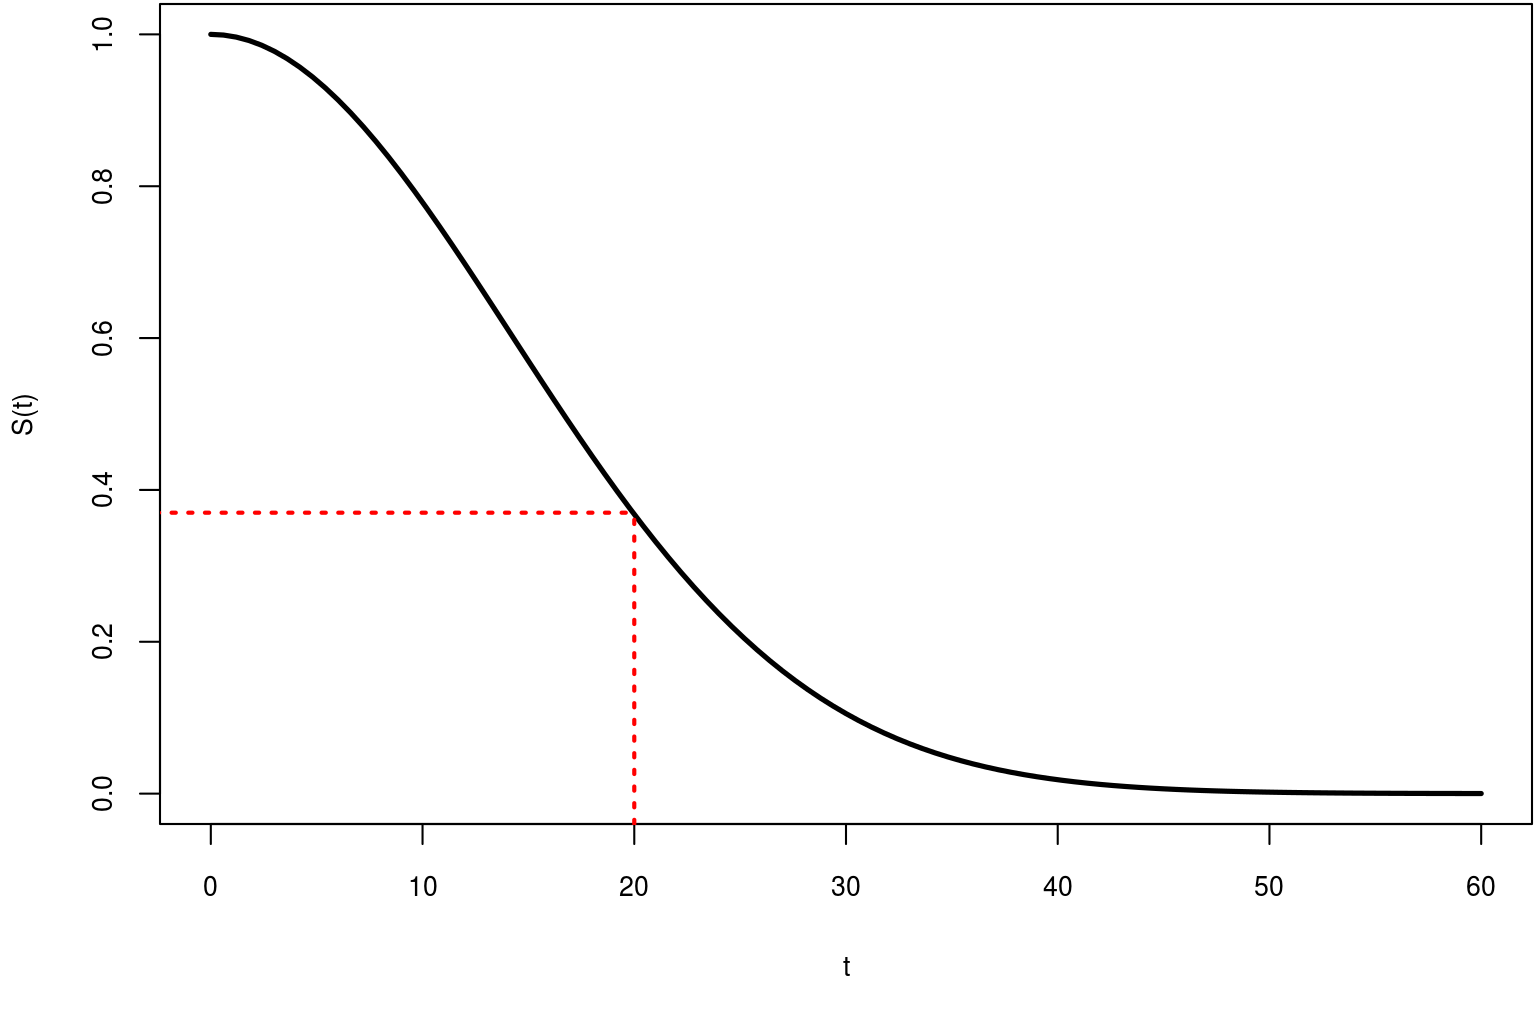
\includegraphics[height=0.8\textheight]{figs/survival_function.png}
\end{frame}

\begin{frame}
\frametitle{Key quantities in survival analysis}
The \textbf{hazard function} (or: hazard rate, failure rate) $h$ is \vspace{-0.2cm}
\begin{align*}
h(t) := & \ \lim_{\Delta t \to 0} \frac{P(t \leq T < t + \Delta t \mid T \geq t)}{\Delta t}.
\end{align*}\vspace{-0.8cm}
\begin{itemize}
\item $h(t) = $ instantaneous failure rate at $t$ given ``survival'' until $t$
\item $h(t)\Delta t$ approximates the probability that $T$ is in the interval $[t, t + \Delta t)$ given $T \geq t$
\item if $T$ corresponds to age at onset, $h(t)$ refers to the incidence rate at age $t$
\end{itemize}

The \textbf{cumulative hazard function} $H$ is given by $H(t) := \int_0^t h(u) du$.

\end{frame}

\begin{frame}
\frametitle{Key quantities in survival analysis}
\centering
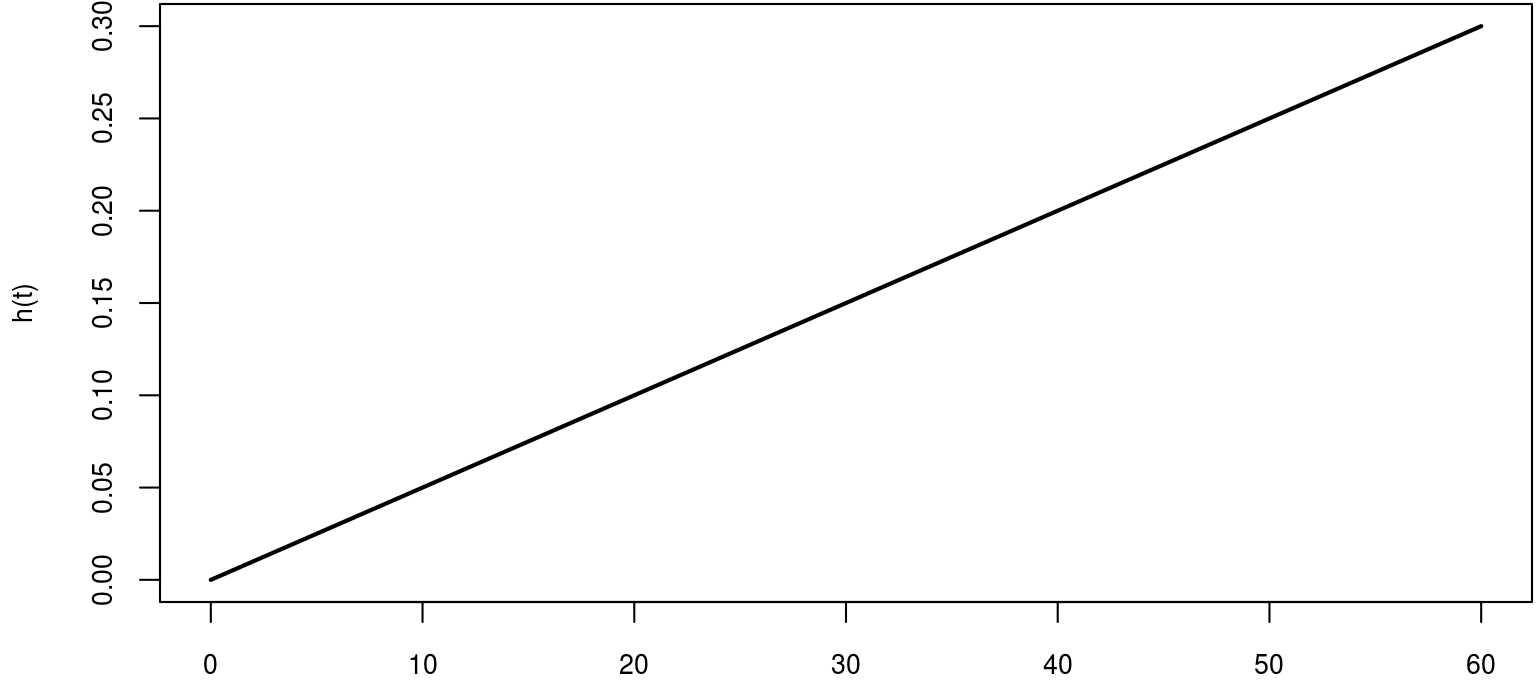
\includegraphics[height=0.4\textheight]{figs/hazard_function.png}

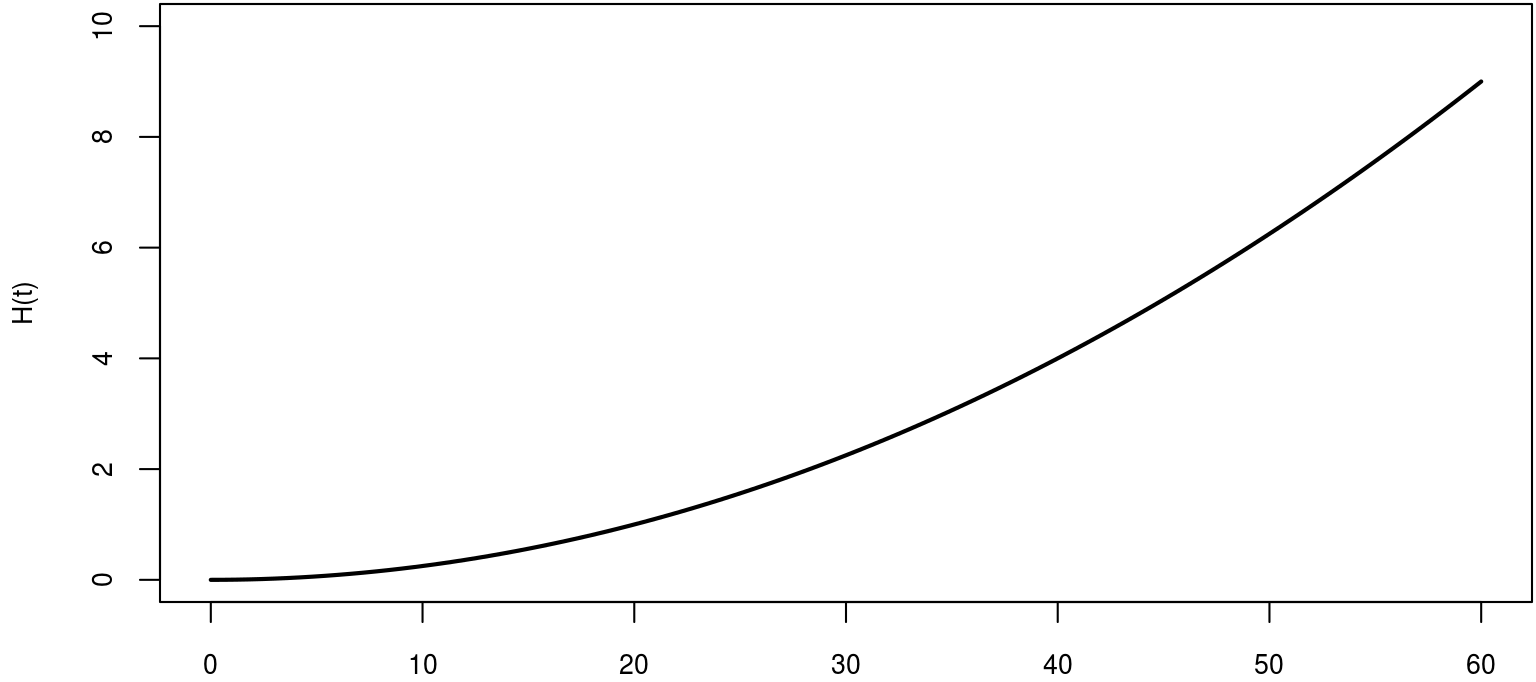
\includegraphics[height=0.4\textheight]{figs/cumulative_hazard_function.png}
\end{frame}

\begin{frame}
\frametitle{Key quantities in survival analysis}
Most methods in survival analysis focus on modeling and/or estimating either the \textcolor{cyan}{survival function} or the \textcolor{Aquamarine}{hazard rate}.

The hazard rate, while somewhat nonintuitive, has some desirable properties:
\begin{itemize}
\item its \textcolor{blue}{conditional interpretation} may be useful in many epidemiological applications
\item it can be \textcolor{blue}{easily estimated using right-censored data}
\end{itemize}
\end{frame}

\begin{frame}
\frametitle{Key quantities in survival analysis}
What shape do we expect the hazard function to have? \textcolor{red}{It depends...}
\begin{enumerate}[(a)]
\item survival from surgery until death due to complications
\item survival from onset of a progressive disease
\item the time before a radioactive atom disintegrates
\item an individual's total lifetime
\end{enumerate}
\begin{center}
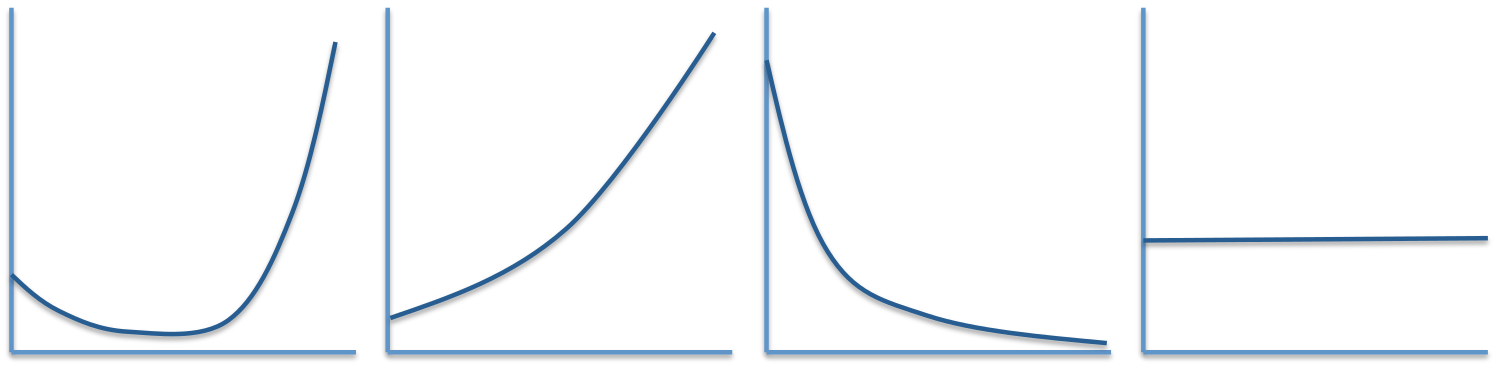
\includegraphics[width = 0.9\textwidth]{figs/hazard_examples.png}

\underline{\,\phantom{right}\,} \hspace{1.5cm} \underline{\,\phantom{right}\,} \hspace{1.5cm} \underline{\,\phantom{right}\,} \hspace{1.5cm} \underline{\,\phantom{right}\,}
\end{center}
\end{frame}

\section{Kaplan-Meier and the log rank test}
\begin{frame}
\frametitle{SECTION 2: KAPLAN-MEIER AND THE LOG RANK TEST}

So far, we have discussed challenges inherent to survival data and some quantities of interest. Now, we will discuss estimating these quantities from right-censored survival data.

For participant $i$, denote by $T_i$ \textbf{the time to event} and by $C_i$ \textbf{the censoring time}. We cannot observe both $T_i$ and $C_i$ -- instead, we observe a pair $(Y_i, \Delta_i)$, where \vspace{-0.3cm}
\begin{itemize}
\item $Y_i := \min(T_i, C_i)$ is the \textbf{observed follow-up time}
\item $\Delta_i = I(T_i \leq C_i)$ is the \textbf{event indicator} [where $I(x = 1)$ is 1 if $x = 1$ and zero otherwise]
\end{itemize}

For example, data represented as $\{7.5, 16.6+, 13.5+, 7.4, 14.2\}$ can now be written as
\[\{(7.5, \underline{\,\phantom{right}\,}), (16.6, \underline{\,\phantom{right}\,}), (13.5, \underline{\,\phantom{right}\,}), (7.4, \underline{\,\phantom{right}\,}), (14.2, \underline{\,\phantom{right}\,})\}.\]
\end{frame}

\begin{frame}
\frametitle{Estimation based on parametric models}

Our goal is generally to \textbf{describe the distribution of} $T$ or some summary of it, and to perform statistical inference to determine if survival differs based on a predictor of interest.

We could, for example, hypothesize that the distribution of $T$ is in a known \textbf{parametric model}, where once we know a parameter (e.g., the mean, standard deviation) we know the whole distribution of $T$.

\end{frame}

\begin{frame}
\frametitle{Estimation based on parametric models}

A variety of parametric families exist, but in survival analysis, the more popular ones are
\begin{itemize}
\item the exponential distribution
\item the Weibull distribution
\item the gamma distribution
\end{itemize}

Each parametric family has characteristics that may or may not make it suitable for the intended application.

However, use of a parametric model comes with a serious risk: \textbf{if the model is misspecified}, the validity of \textbf{our scientific conclusions may be compromised}.
\end{frame}

\begin{frame}
\frametitle{Nonparametric estimation of a survival function}

Suppose we focus on \textbf{estimating the survival probability} $S(t) = P(T > t)$ at time $t$.

If we observed actual survival times $T_1, T_2, \dots, T_n$, we could take
\begin{align*}
\frac{1}{n}\sum_{i=1}^n I(T_i \geq t)
\end{align*}
as an estimator of $S(t)$. This is a \textbf{nonparametric} estimator; we do not have to postulate a parametric model for the true survival distribution.

Can we use this estimator in practice? \pause No, since \textcolor{red}{we do not see $T_i$ for participants who are censored}!
\end{frame}

\begin{frame}
\frametitle{Nonparametric estimation of a survival function}

{\small Denote by $u_1 < u_2 < \dots < u_m$ the observed ordered, distinct times. Also, denote: \vspace{-1cm}

\begin{align*}
d_k = & \ \text{\# of events having occurred at time $u_k$} \\
n_k = & \ \text{\# of individuals at risk at time $u_k$}
\end{align*}
\vspace{-0.5cm}
Suppose the data consist of $\{4, 5, 5+, 8, 12+, 13, 18+, 23, 23, 30\}$.

\begin{center}
\begin{tabular}{|c|c|c|}
\hline
time $u_k$ & $d_k$ & $n_k$ \\
\hline
4 & 1 & 10 \\
5 & 1 & 9 \\
8 & 1 & 7 \\
12 & 0 & 6 \\
13 & 1 & 5 \\
18 & 0 & 4 \\
23 & 2 & 3 \\
30 & 1 & 1 \\
\hline
\end{tabular}
\end{center}
}
\end{frame}

\begin{frame}
\frametitle{Nonparametric estimation of a survival function}

{\small Suppose the data consist of $\{4, 5, 5+, 8, 12+, 13, 18+, 23, 23, 30\}$.}

\begin{center}
\begin{tabular}{|c|c|c|}
\hline
time $u_k$ & $d_k$ & $n_k$ \\
\hline
4 & 1 & 10 \\
5 & 1 & 9 \\
8 & 1 & 7 \\
12 & 0 & 6 \\
13 & 1 & 5 \\
18 & 0 & 4 \\
23 & 2 & 3 \\
30 & 1 & 1 \\
\hline
\end{tabular}
\end{center}

Is $m$ the number of events in the sample? \underline{\;\;\phantom{right}\;\;}

When does $m = n$? \underline{\;\;\phantom{right}\;\;}
\end{frame}

\begin{frame}
\frametitle{Nonparametric estimation of a survival function}

What is a sensible estimate of $P(T > u_1)$?

$P(T > u_1) = P(T > u_1 \mid T \geq u_1)P(T \geq u_1) \approx \underline{\;\;\;\phantom{right}\;\;\;}$ \pause

What is a sensible estimate of $P(T > u_2)$?
\begin{align*}
P(T > u_2) =& \ P(T > u_2 \mid T \geq u_2)P(T \geq u_2) \\
\approx &\ P(T > u_2 \mid T \geq u_2)P(T > u_1) \approx \underline{\;\;\;\phantom{right}\;\;\;}
\end{align*} \pause

What is a sensible estimate of $P(T > u_3)$? \pause
\begin{align*}
P(T > u_3) =& \ P(T > u_3 \mid T \geq u_3)P(T \geq u_3) \\
\approx &\ P(T > u_3 \mid T \geq u_3)P(T > u_2) \approx \underline{\;\;\;\phantom{right}\;\;\;}
\end{align*}

\end{frame}

\begin{frame}
\frametitle{Nonparametric estimation of a survival function}
Continuing in this fashion yields the \textbf{Kaplan-Meier} estimator of $S(t)$: \vspace{-0.3cm}
\begin{align*}
\widehat{S}(t) := \prod_{k: u_k \leq t} \left(1 - \frac{d_k}{n_k} \right).
\end{align*}\vspace{-0.5cm}

If any participant is censored at $u_m$, we consider $\widehat{S}(t)$ to be undefined for $t > u_m$. (remember, $u_m$ is the maximum time)

A few observations:
\begin{itemize}
\item $\widehat{S}(t) = 1$ for each $t$ preceding the first event time $u_1$ \pause
\item $\widehat{S}$ is a non-increasing function. Why? \pause
\item $\widehat{S}$ drops to zero at the largest time $u_m$ only if \underline{\;\;\;\;\phantom{right}\;\;\;} \pause
\item the KM estimator only jumps at observed event times \pause
\item the KM estimator relies on \textbf{independent censoring} but does not require postulating a parametric family, and is thus \textbf{nonparametric}
\end{itemize}
\end{frame}

\begin{frame}
\frametitle{Nonparametric estimation of a survival function}

\hspace*{-0.5cm}\begin{tabular}{|c|c|c|c|c|c|}
\hline
time $u_k$ & $d_k$ & $n_k$ & $d_k/n_k$ & $1 - d_k/n_k$ & $\widehat{S}(u_k)$ \\
\hline
4 & 1 & 10 & 0.1 & \textcolor{Aquamarine}{0.9} & $1 \times \textcolor{Aquamarine}{0.9} = \textcolor{blue}{0.9}$\\
5 & 1 & 9 & 0.1111 & \textcolor{Aquamarine}{0.8888} & $0.9 \times \textcolor{Aquamarine}{0.8888} = \textcolor{blue}{0.8}$ \\
8 & 1 & 7 & 0.1429 & \textcolor{Aquamarine}{0.8571} & $0.8 \times \textcolor{Aquamarine}{0.8571} = \textcolor{blue}{0.6857}$\\
12 & 0 & 6 & 0 & \textcolor{Aquamarine}{1} & $0.6857 \times \textcolor{Aquamarine}{1} = \textcolor{blue}{0.6857}$\\
13 & 1 & 5 & 0.2 & \textcolor{Aquamarine}{0.8} & $0.6857 \times \textcolor{Aquamarine}{0.8} = \textcolor{blue}{0.5486}$\\
18 & 0 & 4 & 0 & \textcolor{Aquamarine}{1} & $0.5846 \times \textcolor{Aquamarine}{1} = \textcolor{blue}{0.5486}$\\
23 & 2 & 3 & 0.666 & \textcolor{Aquamarine}{0.3333} & $0.5486 \times \textcolor{Aquamarine}{0.3333} = \textcolor{blue}{0.1829}$\\
30 & 1 & 1 & 1 & \textcolor{Aquamarine}{0} & $0.1829 \times \textcolor{Aquamarine}{0} = \textcolor{blue}{0}$\\
\hline
\end{tabular}
\end{frame}

\begin{frame}
\frametitle{Nonparametric estimation of a survival function}
\centering
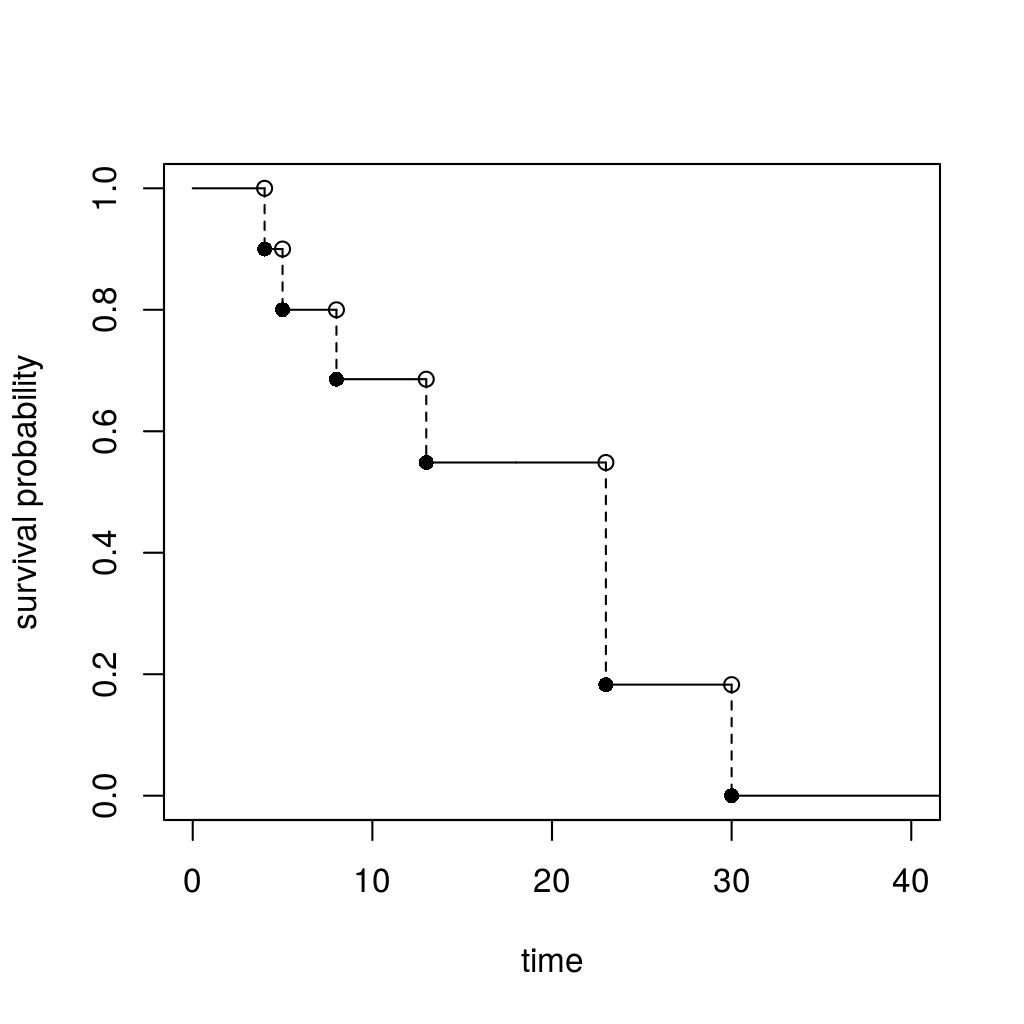
\includegraphics[width=0.8\textwidth]{figs/km_small_example.png}
\end{frame}

\begin{frame}
\frametitle{Nonparametric estimation of a survival function}

Our estimate of $\widehat{S}(t)$ has a corresponding standard error,
\begin{align*}
\widehat{SE}(t) := \widehat{S}(t)\sqrt{\sum_{i : u_i \leq t}\frac{d_i}{n_i(n_i - d_i)}}.
\end{align*}
This suggests using 
\textcolor{blue}{[$\widehat{S}(t) - 1.96 \widehat{SE}(t)$, $\widehat{S}(t) + 1.96 \widehat{SE}(t)$]} as a 95\% confidence interval for $S(t)$.

As before, \textbf{\texttt{R} can calculate these for you.}
\end{frame}

\begin{frame}
\frametitle{Nonparametric estimation of a survival function}
\begin{tabular}{|c|c|c|c|c|c|c|}
\hline
time $u_k$ & $d_k$ & $n_k$ & $\widehat{S}(u_k)$ & $\widehat{SE}(t)$ & left limit & right limit \\
\hline
4 & 1 & 10 & 0.9 & 0.0949 & \textcolor{Aquamarine}{0.7141} & \textcolor{red}{1.0859} \\
5 & 1 & 9 &  0.8 & 0.0949 & \textcolor{Aquamarine}{0.5521} & \textcolor{red}{1.0479}\\
8 & 1 & 7 & 0.6857 & 0.0949 & \textcolor{Aquamarine}{0.3888} & \textcolor{Aquamarine}{0.9826}\\
12 & 0 & 6 & 0.6857 & 0.0949 & \textcolor{Aquamarine}{0.3888} & \textcolor{Aquamarine}{0.9826}\\
13 & 1 & 5 & 0.5486 & 0.0949 & \textcolor{Aquamarine}{0.2106} & \textcolor{Aquamarine}{0.8866}\\
18 & 0 & 4 & 0.5486 & 0.0949 & \textcolor{Aquamarine}{0.2106} & \textcolor{Aquamarine}{0.8866}\\
23 & 2 & 3 & 0.1829 & 0.0949 & \textcolor{red}{-0.1307} & \textcolor{Aquamarine}{0.4965}\\
30 & 1 & 1 & 0 & & & \\
\hline
\end{tabular}
\end{frame}

\begin{frame}
\frametitle{Nonparametric estimation of a survival function}
\centering
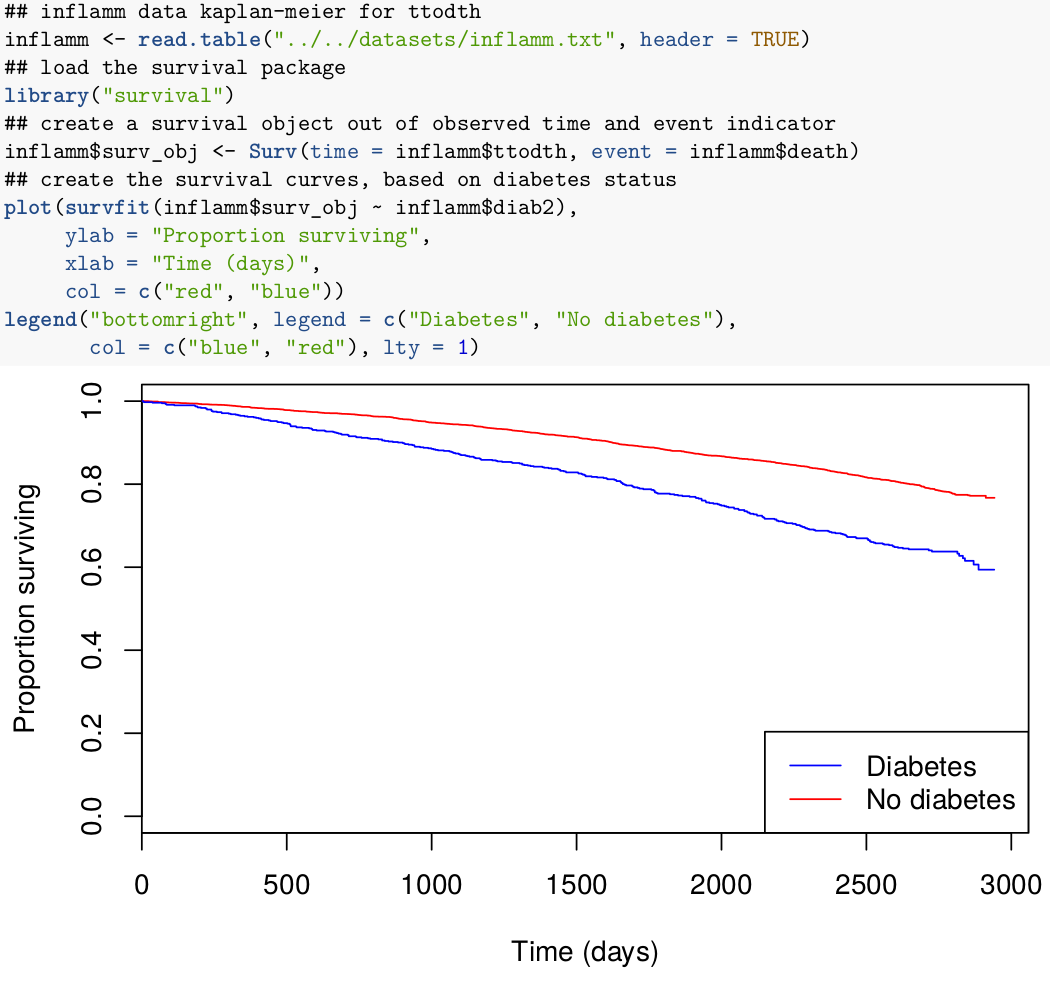
\includegraphics[height=0.95\textheight]{figs/inflamm_km.png}
\end{frame}

\begin{frame}
\frametitle{Nonparametric estimation of a survival function}
\centering
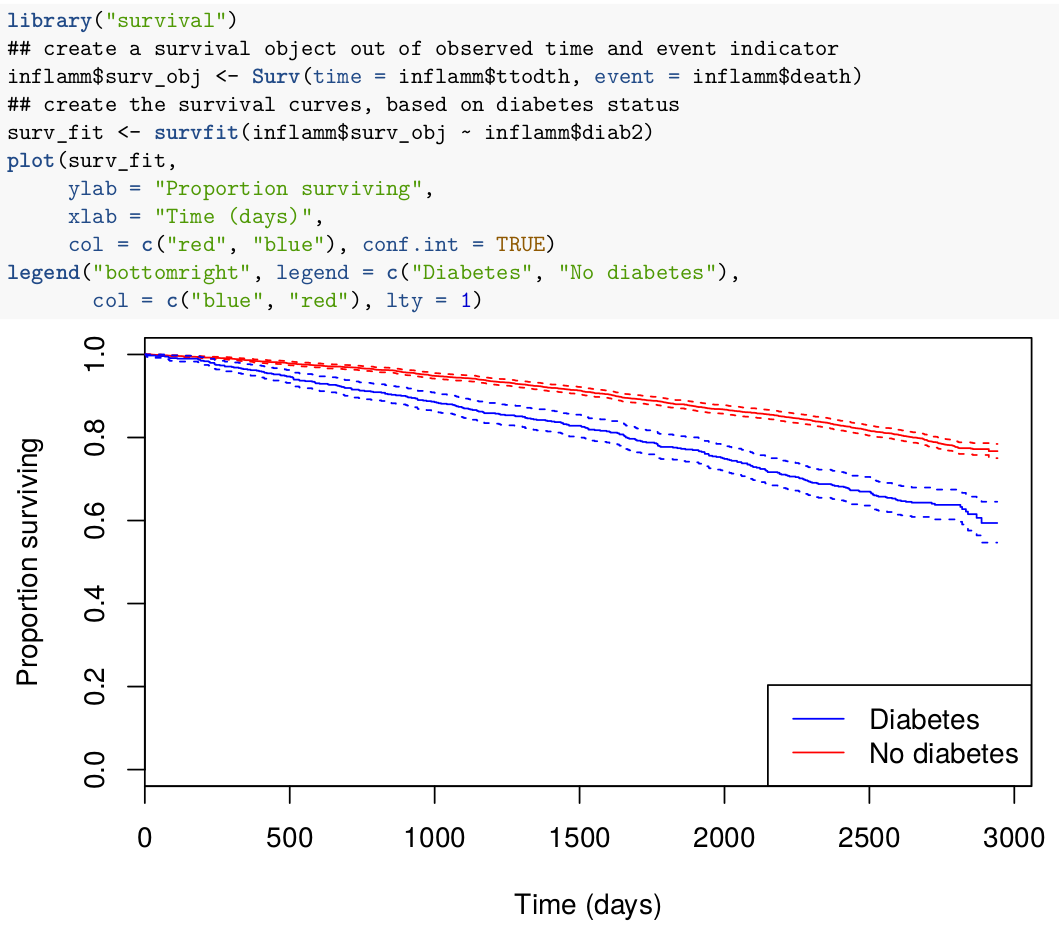
\includegraphics[height=0.95\textheight]{figs/inflamm_km_cis.png}
\end{frame}

\begin{frame}
\frametitle{Nonparametric estimation of measures of central tendency}

With continuous or binary data, we often used the mean or median to describe the distribution of the variable.

Can we describe the \textbf{central tendency of a distribution} using right-censored data?

Should we (or can we) use the \textbf{mean} or the \textbf{median}?
\begin{itemize}
\item the mean may be simpler to communicate
\item the median is robust to outliers, while the mean is not
\item in survival analysis, the mean can be problematic because \textcolor{red}{censoring may render the right tail of the distribution unestimable}
\end{itemize}
\end{frame}

\begin{frame}
\frametitle{Nonparametric estimation of measures of central tendency}

For this reason, people tend to focus on the \textbf{restricted mean} $\mu_\tau := \int_0^\tau S(u) du$; an estimator is given by $\widehat{\mu}_\tau := \int_0^\tau \widehat{S}(u)du$.

\textcolor{red}{However, the interpretation of $\mu_\tau$ may not be of interest}, leading people to consider the median instead.

Whenever $S$ is continuous and strictly decreasing, we define the median as the \textbf{timepoint $t_{0.5}$ such that $S(t_{0.5}) = 1/2$}.
\end{frame}

\begin{frame}
\frametitle{Nonparametric estimation of measures of central tendency}
\centering
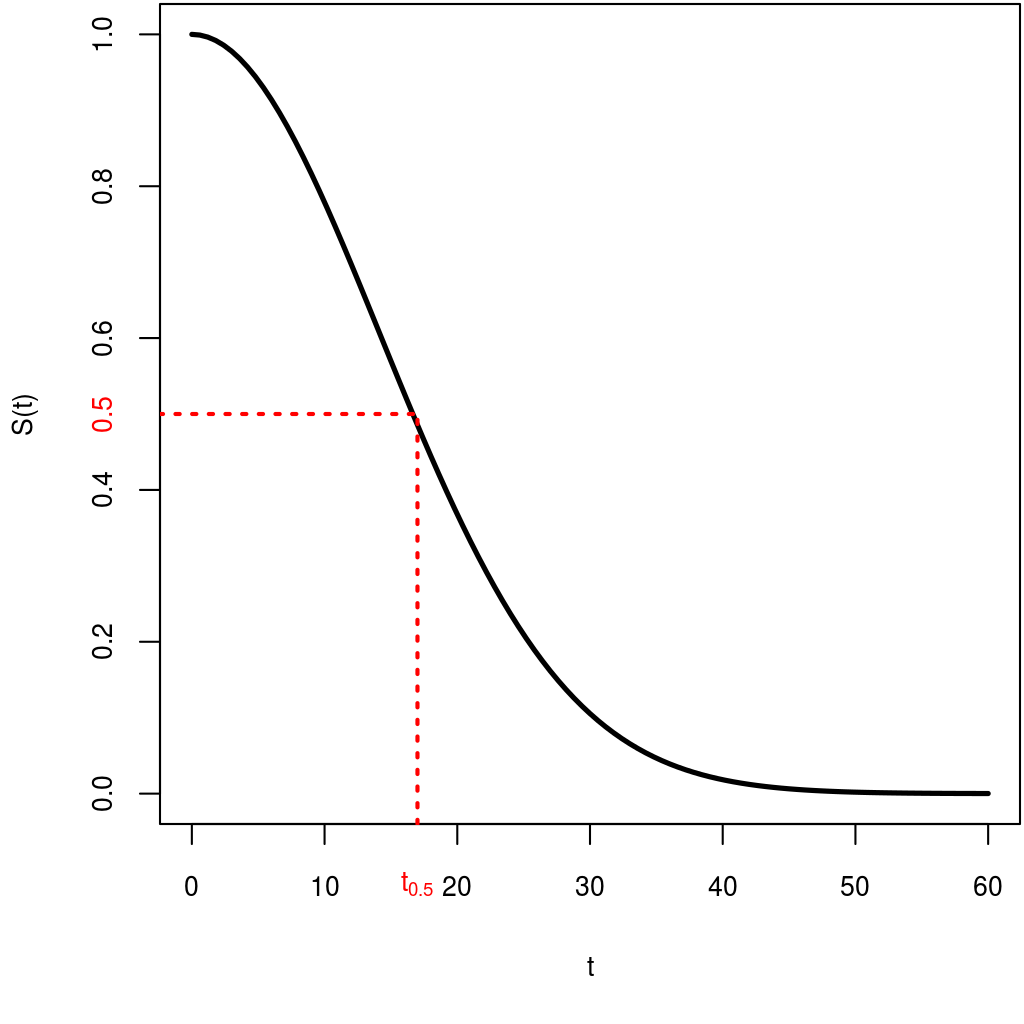
\includegraphics[width=0.8\textheight]{figs/survival_function_median.png}
\end{frame}

\begin{frame}
\frametitle{Nonparametric estimation of measures of central tendency}
In practice, we will use as estimator of $t_{0.5}$ the median $\hat{t}_{0.5}$ of $\widehat{S}$. But the survival function $\widehat{S}$ is \textbf{not continuous nor strictly decreasing}!

\begin{center}
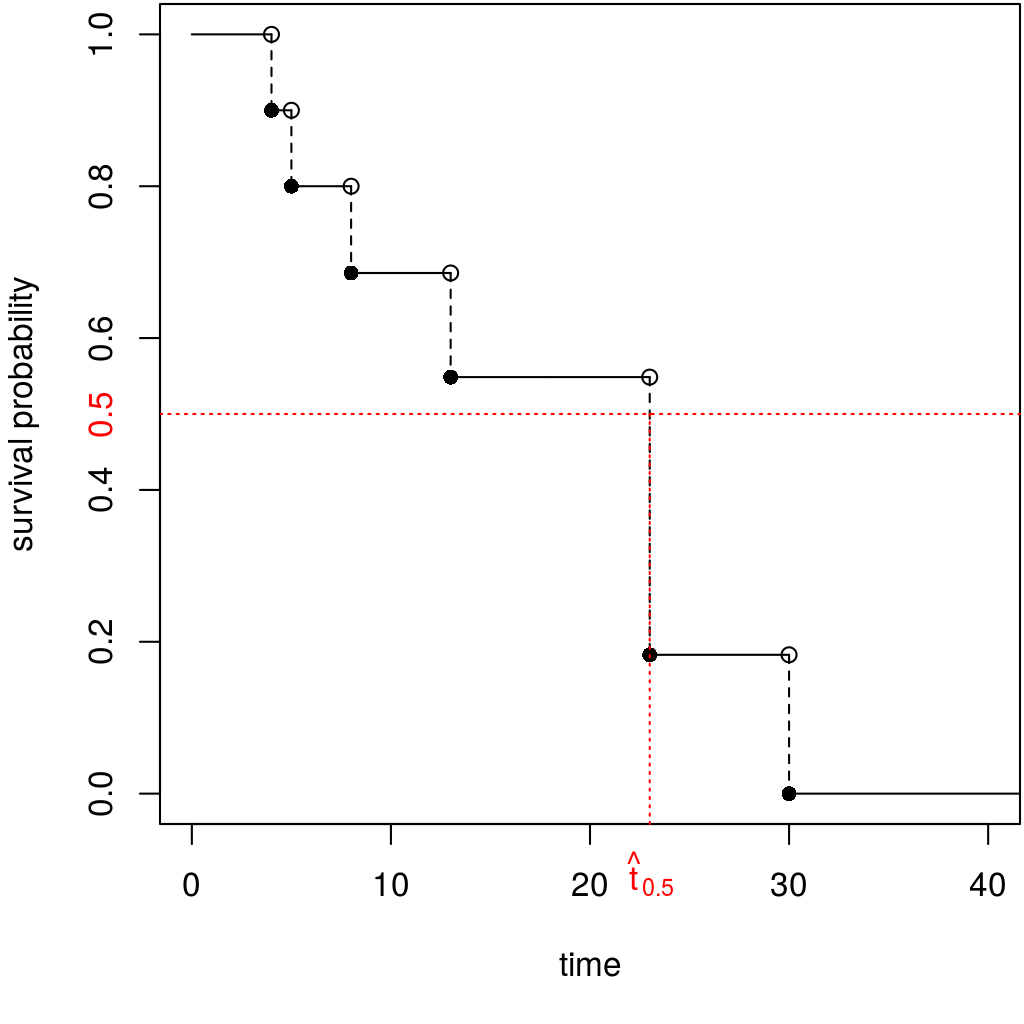
\includegraphics[width=0.6\textheight]{figs/km_small_example_median.png}
\end{center}
\end{frame}


\begin{frame}
\frametitle{Nonparametric estimation of measures of central tendency}
Close or put away your notes and laptops. Then answer the following questions, paying attention your thought process (you will hand in your responses):
\begin{enumerate}
\item What if there is no point $\hat{t}_{0.5}$ at which $\widehat{S}$ goes from above to below 0.5?
\item What happens if $\widehat{S}$ equals 0.5 over a whole interval?
\end{enumerate}

\end{frame}

\begin{comment}
\begin{frame}
\frametitle{Nonparametric estimation of measures of central tendency}
\begin{enumerate}
\item What if there is no point $\hat{t}_{0.5}$ at which $\widehat{S}$ goes from above to below 0.5?
\item[] \textcolor{blue}{Then we cannot estimate the median survival time!}
\item What happens if $\widehat{S}$ equals 0.5 over a whole interval?
\item[] \textcolor{blue}{Then we should pick the smallest value $t$ such that $\widehat{S}(t) \leq 0.5$ (no one has the event in this range by definition)}
\end{enumerate}

\end{frame}
\end{comment}

\begin{frame}
\frametitle{Nonparametric testing of equal survivorship between two groups}

It is often of interest to \textbf{contrast the survivorship of several groups}, rather than simply describing the survival time distribution in a single group. For example:
\begin{itemize}
\item Does time to death depend on diabetes status?
\item Does treatment for leukemia affect time in remission?
\end{itemize}

Commonly, in survival analysis, we \textcolor{blue}{compare the entire survival function between two groups} to make this contrast.
\end{frame}

\begin{frame}
\frametitle{Nonparametric testing of equal survivorship between two groups}

Comparing the entire survival function is the same as saying that the group-specific time-to-event distributions are identical. Thus, we are testing (for two groups denoted by $Z = 0$ and $Z = 1$)
\begin{align*}
\textcolor{Aquamarine}{H_0: S_0(t) = S_1(t) \text{ for all } t} \ \text{vs} \ \textcolor{BurntOrange}{H_a: S_0(t) \neq S_1(t) \text{ for some }t}.
\end{align*}
At any observed failure time $t$, we can construct a $2 \times 2$ table:\vspace{-0.2cm}

\begin{center}
\begin{tabular}{c|c|c|c}
& $Z = 0$ & $Z = 1$ \\
\hline
died & $d_0(t)$ & $d_1(t)$ & $d(t)$ \\
did not die & $s_0(t)$ & $s_1(t)$ & $s(t)$\\
at risk & $n_0(t)$ & $n_1(t)$ & $n(t)$
\end{tabular}
\end{center}\vspace{-0.2cm}

If $H_0$ is true, then we expect that the row/column classifications are independent, and thus that $\frac{d_0(t)}{n_0(t)} \approx \frac{d_1(t)}{n_1(t)}$.
\end{frame}

\begin{frame}
\frametitle{Nonparametric testing of equal survivorship between two groups}

\begin{center}
\begin{tabular}{c|c|c|c}
& $Z = 0$ & $Z = 1$ \\
\hline
died & $d_0(t)$ & $d_1(t)$ & $d(t)$ \\
did not die & $s_0(t)$ & $s_1(t)$ & $s(t)$\\
at risk & $n_0(t)$ & $n_1(t)$ & $n(t)$
\end{tabular}
\end{center}\vspace{-0.2cm}

With the table margins fixed, what do we expect to see in the top-left cell under $H_0$?
\begin{align*}
\textbf{observed count } o(t) = & \ d_0(t) \\
\textbf{expected count } e(t) = & \ \frac{d(t)}{n(t)}\times \frac{n_0(t)}{n(t)}n(t) = \frac{d(t)n_0(t)}{n(t)}
\end{align*}
\textcolor{Aquamarine}{The difference $o(t) - e(t)$ should be small under $H_0$.} 
\end{frame}

\begin{frame}
\frametitle{Nonparametric testing of equal survivorship between two groups}
Conditional on the margins, and under $H_0$, this difference has variance equal to $v(t) := \frac{n_0(t)n_1(t)d(t)s(t)}{n(t)^2\{n(t) - 1\}}$.

We can aggregate $o(t) - e(t)$ over \textcolor{BurntOrange}{all distinct observed failure times} to get the \textbf{logrank test statistic}
\begin{align*}
\widehat{T}^2_{LR, n} := \left[\frac{\sum_i \{o(t_i) - e(t_i)\}}{\sqrt{\sum_i}v(t_i)} \right]^2,
\end{align*}
which is an adaptation of the Mantel-Cochran-Haenszel test (for matched pairs data) for survival data.

\textcolor{cyan}{Under $H_0$, with large sample size the distribution of $\widehat{T}^2_{LR, n}$ is approximately $\chi^2_1$}: thus, if we observe $\widehat{T}^2_{LR, n} = x$, then the p-value is given by $P(\chi^2_1 > x)$!
\end{frame}

\begin{frame}
\frametitle{Nonparametric testing of equal survivorship between two groups}

\centering
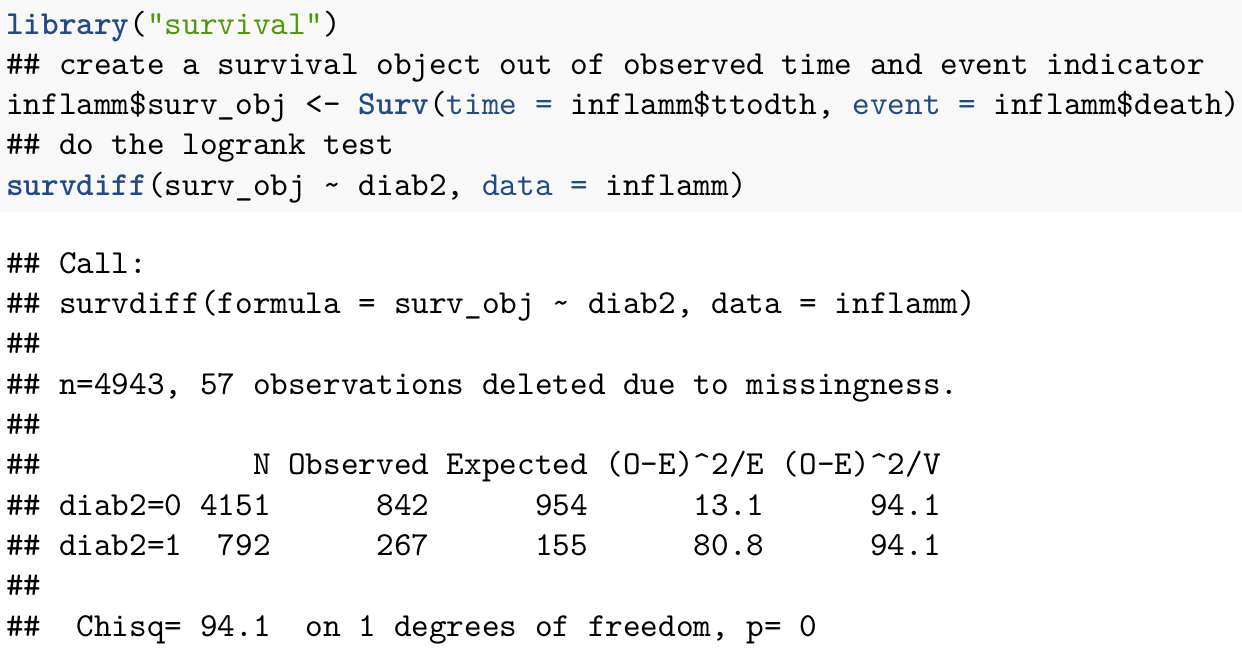
\includegraphics[width=1\textwidth]{figs/inflamm_logrank.png}
\end{frame}

\begin{frame}[fragile]
\frametitle{Motivation for regression modeling}

\textcolor{red}{What about potential confounders?} \pause

It is \textcolor{BurntOrange}{possible} to adapt the logrank test, by breaking up the potential confounder into discrete categories, computing the observed and expected counts within each stratum, and then summing over the strata. \textbf{\texttt{R} will do this for us}, using the same notation to add confounders as before:\vspace{-0.3cm} 
\begin{verbatim}
survdiff(Y ~ X_1 + X_2 + \dots, data = \dots)
\end{verbatim}\vspace{-0.5cm}

However, regression modeling may be more useful in some settings, by: \vspace{-0.3cm}
\begin{itemize}
\item \textbf{borrowing information} across subgroups
\item \textbf{summarizing} the relative survival experience of different subgroups in a \textcolor{blue}{single summary measure}
\end{itemize}
\end{frame}

\section{Semiparametric estimation and inference}
\begin{frame}
\frametitle{SECTION 3: COX PROPORTIONAL HAZARDS REGRESSION}

\end{frame}

\begin{comment}
% cox ph regression, assumptions
\section{Summary}
\begin{frame}
\frametitle{SECTION 4: SUMMARY}
\end{frame}
% different ways to look at survival data
\end{comment}
\end{document}